\documentclass[a4paper,landscape]{article}\usepackage[]{graphicx}\usepackage[]{color}
%% maxwidth is the original width if it is less than linewidth
%% otherwise use linewidth (to make sure the graphics do not exceed the margin)
\makeatletter
\def\maxwidth{ %
  \ifdim\Gin@nat@width>\linewidth
    \linewidth
  \else
    \Gin@nat@width
  \fi
}
\makeatother

\definecolor{fgcolor}{rgb}{0.345, 0.345, 0.345}
\newcommand{\hlnum}[1]{\textcolor[rgb]{0.686,0.059,0.569}{#1}}%
\newcommand{\hlstr}[1]{\textcolor[rgb]{0.192,0.494,0.8}{#1}}%
\newcommand{\hlcom}[1]{\textcolor[rgb]{0.678,0.584,0.686}{\textit{#1}}}%
\newcommand{\hlopt}[1]{\textcolor[rgb]{0,0,0}{#1}}%
\newcommand{\hlstd}[1]{\textcolor[rgb]{0.345,0.345,0.345}{#1}}%
\newcommand{\hlkwa}[1]{\textcolor[rgb]{0.161,0.373,0.58}{\textbf{#1}}}%
\newcommand{\hlkwb}[1]{\textcolor[rgb]{0.69,0.353,0.396}{#1}}%
\newcommand{\hlkwc}[1]{\textcolor[rgb]{0.333,0.667,0.333}{#1}}%
\newcommand{\hlkwd}[1]{\textcolor[rgb]{0.737,0.353,0.396}{\textbf{#1}}}%

\usepackage{framed}
\makeatletter
\newenvironment{kframe}{%
 \def\at@end@of@kframe{}%
 \ifinner\ifhmode%
  \def\at@end@of@kframe{\end{minipage}}%
  \begin{minipage}{\columnwidth}%
 \fi\fi%
 \def\FrameCommand##1{\hskip\@totalleftmargin \hskip-\fboxsep
 \colorbox{shadecolor}{##1}\hskip-\fboxsep
     % There is no \\@totalrightmargin, so:
     \hskip-\linewidth \hskip-\@totalleftmargin \hskip\columnwidth}%
 \MakeFramed {\advance\hsize-\width
   \@totalleftmargin\z@ \linewidth\hsize
   \@setminipage}}%
 {\par\unskip\endMakeFramed%
 \at@end@of@kframe}
\makeatother

\definecolor{shadecolor}{rgb}{.97, .97, .97}
\definecolor{messagecolor}{rgb}{0, 0, 0}
\definecolor{warningcolor}{rgb}{1, 0, 1}
\definecolor{errorcolor}{rgb}{1, 0, 0}
\newenvironment{knitrout}{}{} % an empty environment to be redefined in TeX

\usepackage{alltt}
\usepackage{geometry}
\usepackage{graphicx}
\usepackage{tikz}
\IfFileExists{upquote.sty}{\usepackage{upquote}}{}
\begin{document}









\begin{knitrout}
\definecolor{shadecolor}{rgb}{0.969, 0.969, 0.969}\color{fgcolor}
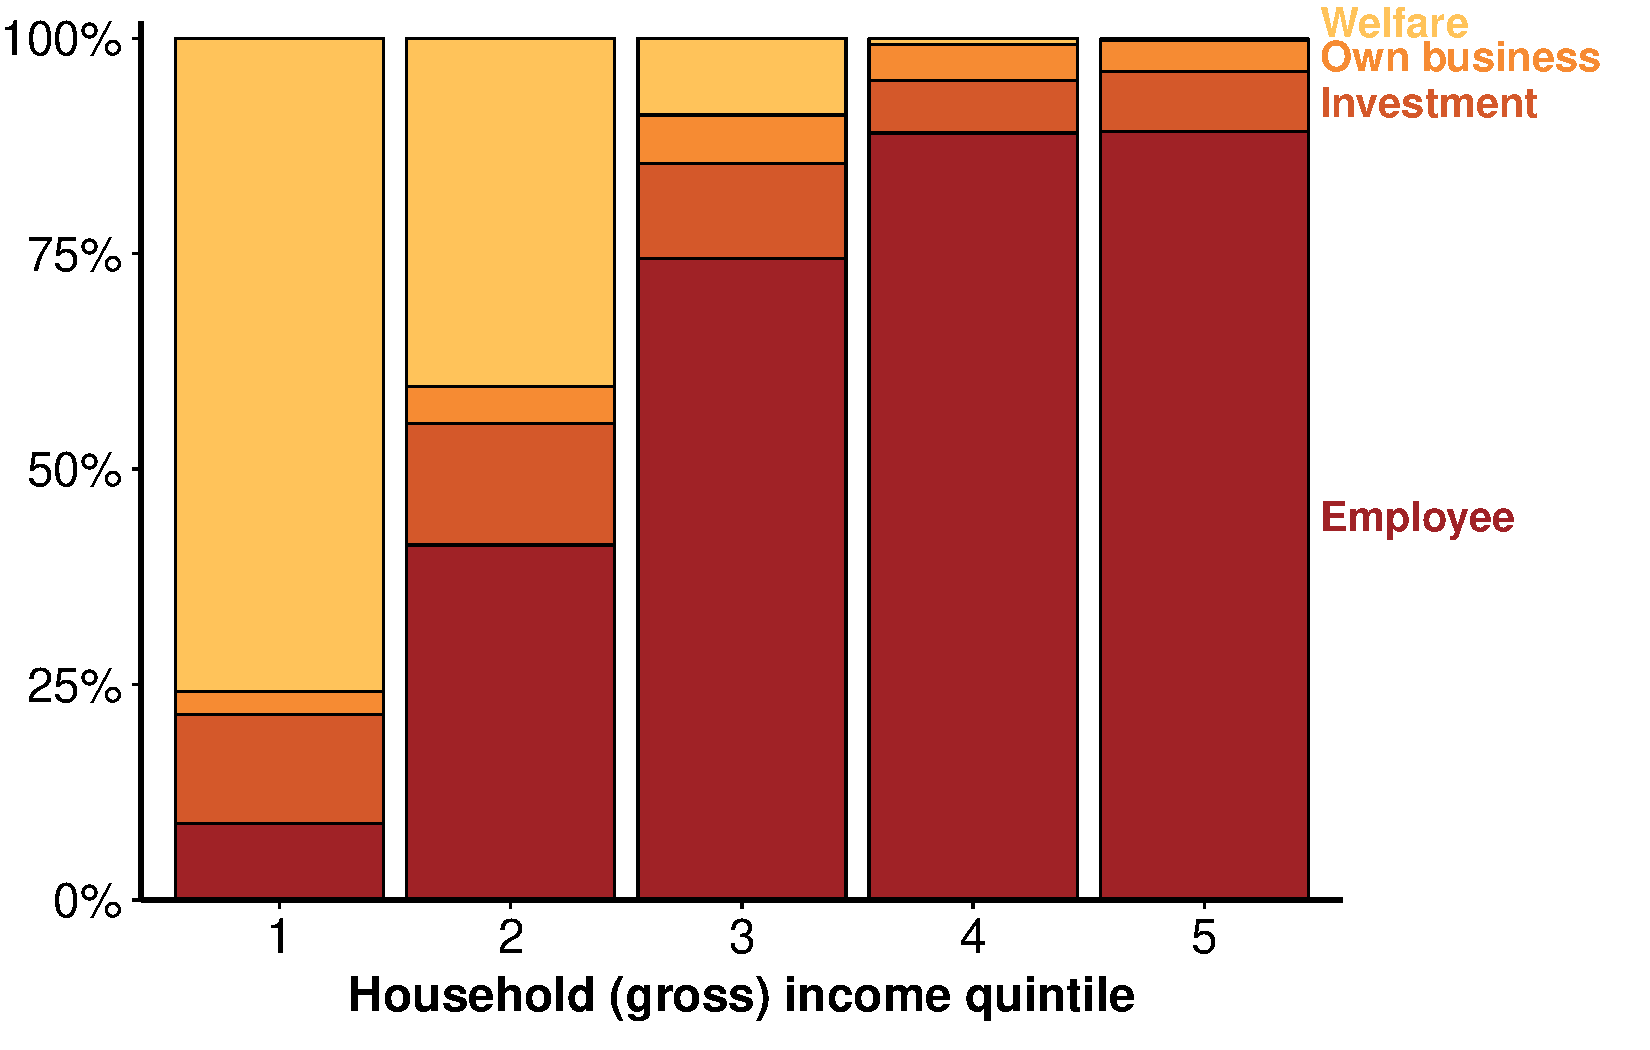
\includegraphics[width=11.000in,height=7.00in]{figure/GST-Figure-5-1} 

\end{knitrout}

\begin{knitrout}
\definecolor{shadecolor}{rgb}{0.969, 0.969, 0.969}\color{fgcolor}
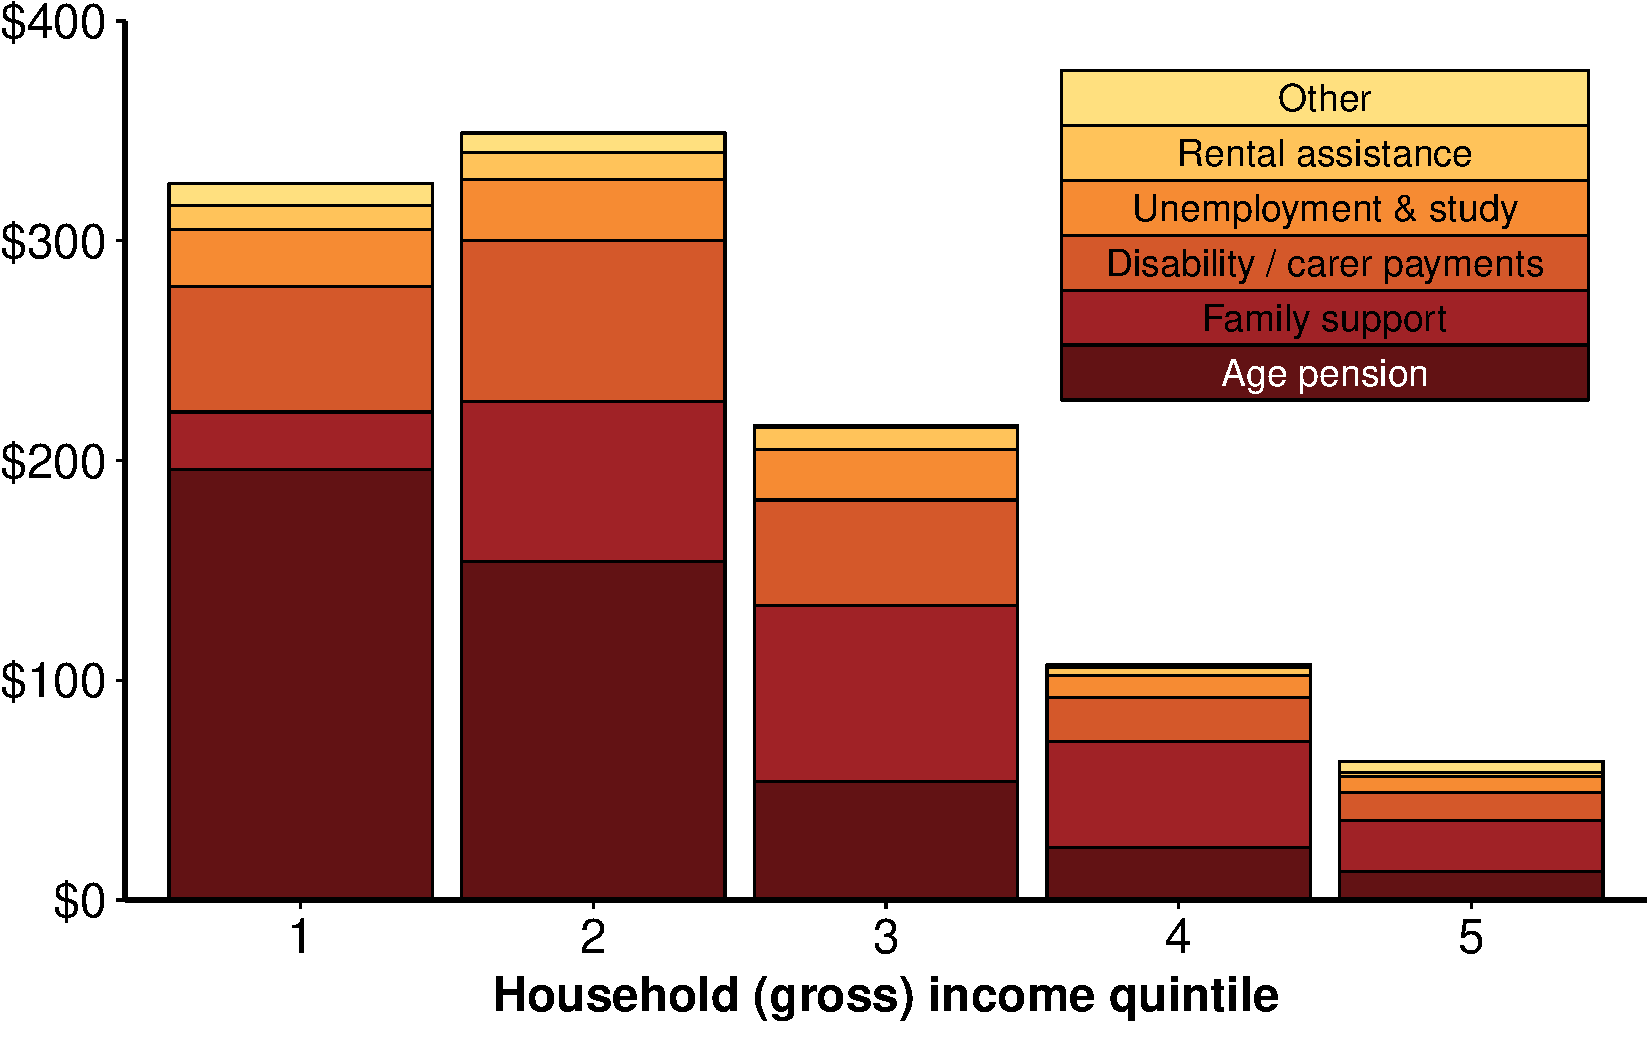
\includegraphics[width=11.000in,height=7.00in]{figure/GST-Figure-6-1} 

\end{knitrout}

\begin{knitrout}
\definecolor{shadecolor}{rgb}{0.969, 0.969, 0.969}\color{fgcolor}
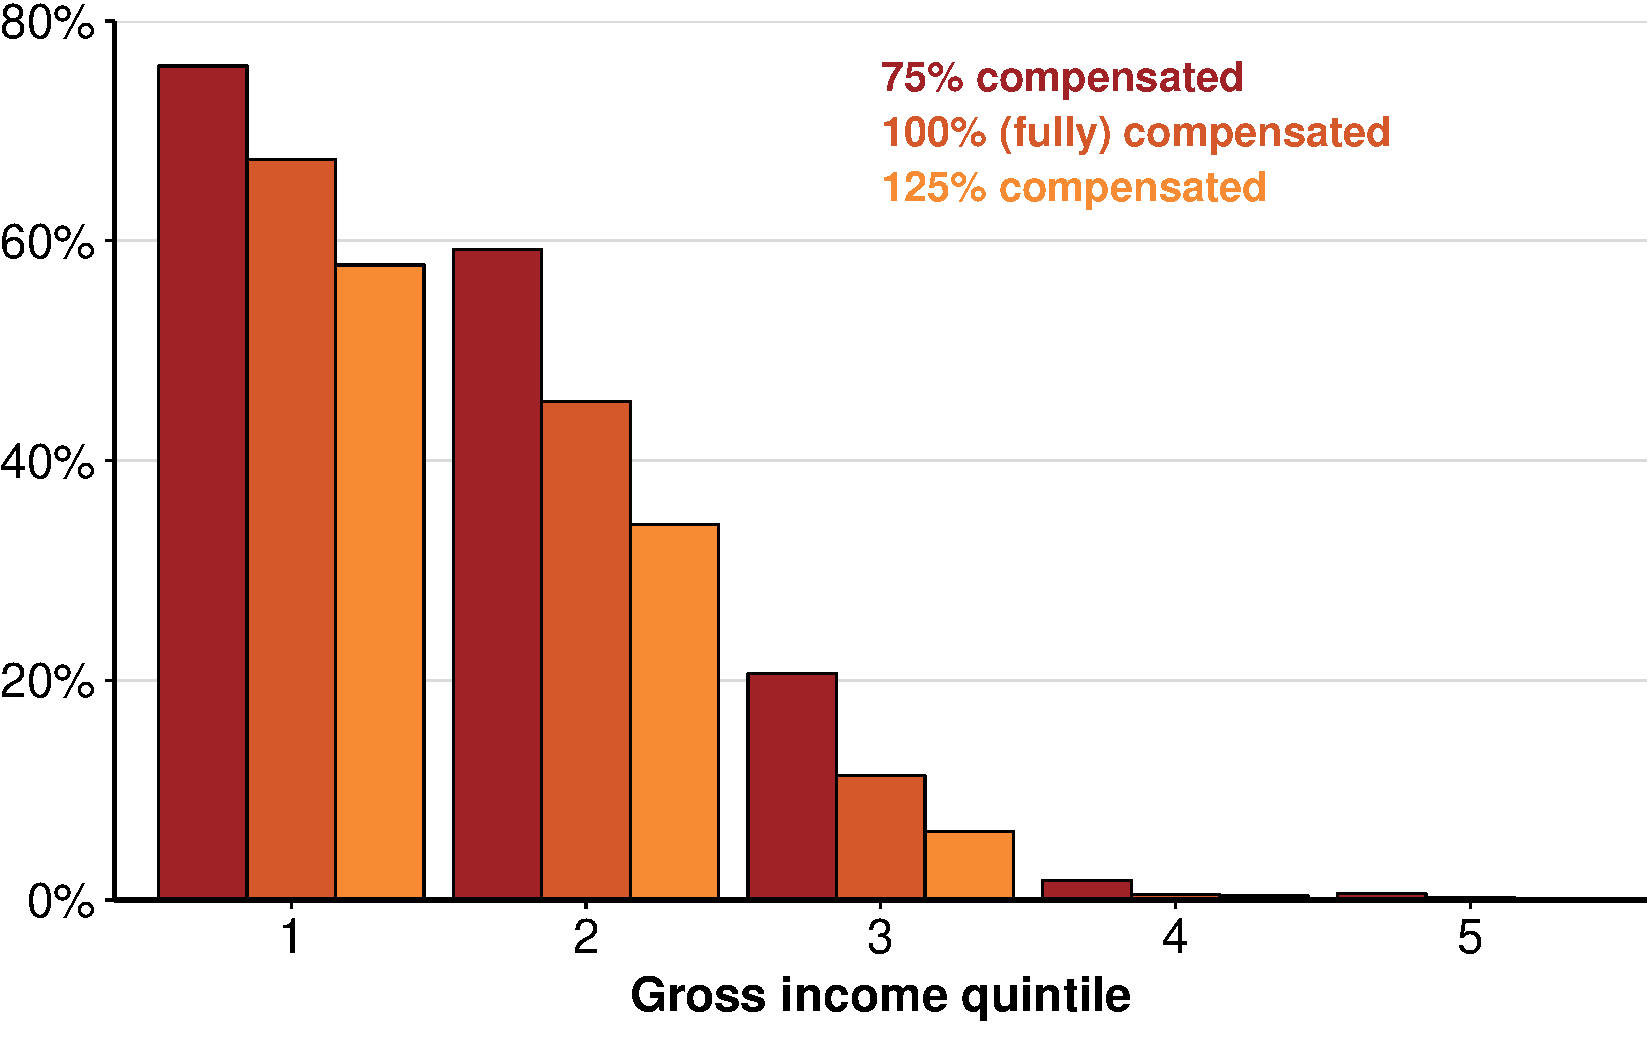
\includegraphics[width=11.000in,height=7.00in]{figure/GST-Figure-7-1} 

\end{knitrout}

\begin{knitrout}
\definecolor{shadecolor}{rgb}{0.969, 0.969, 0.969}\color{fgcolor}
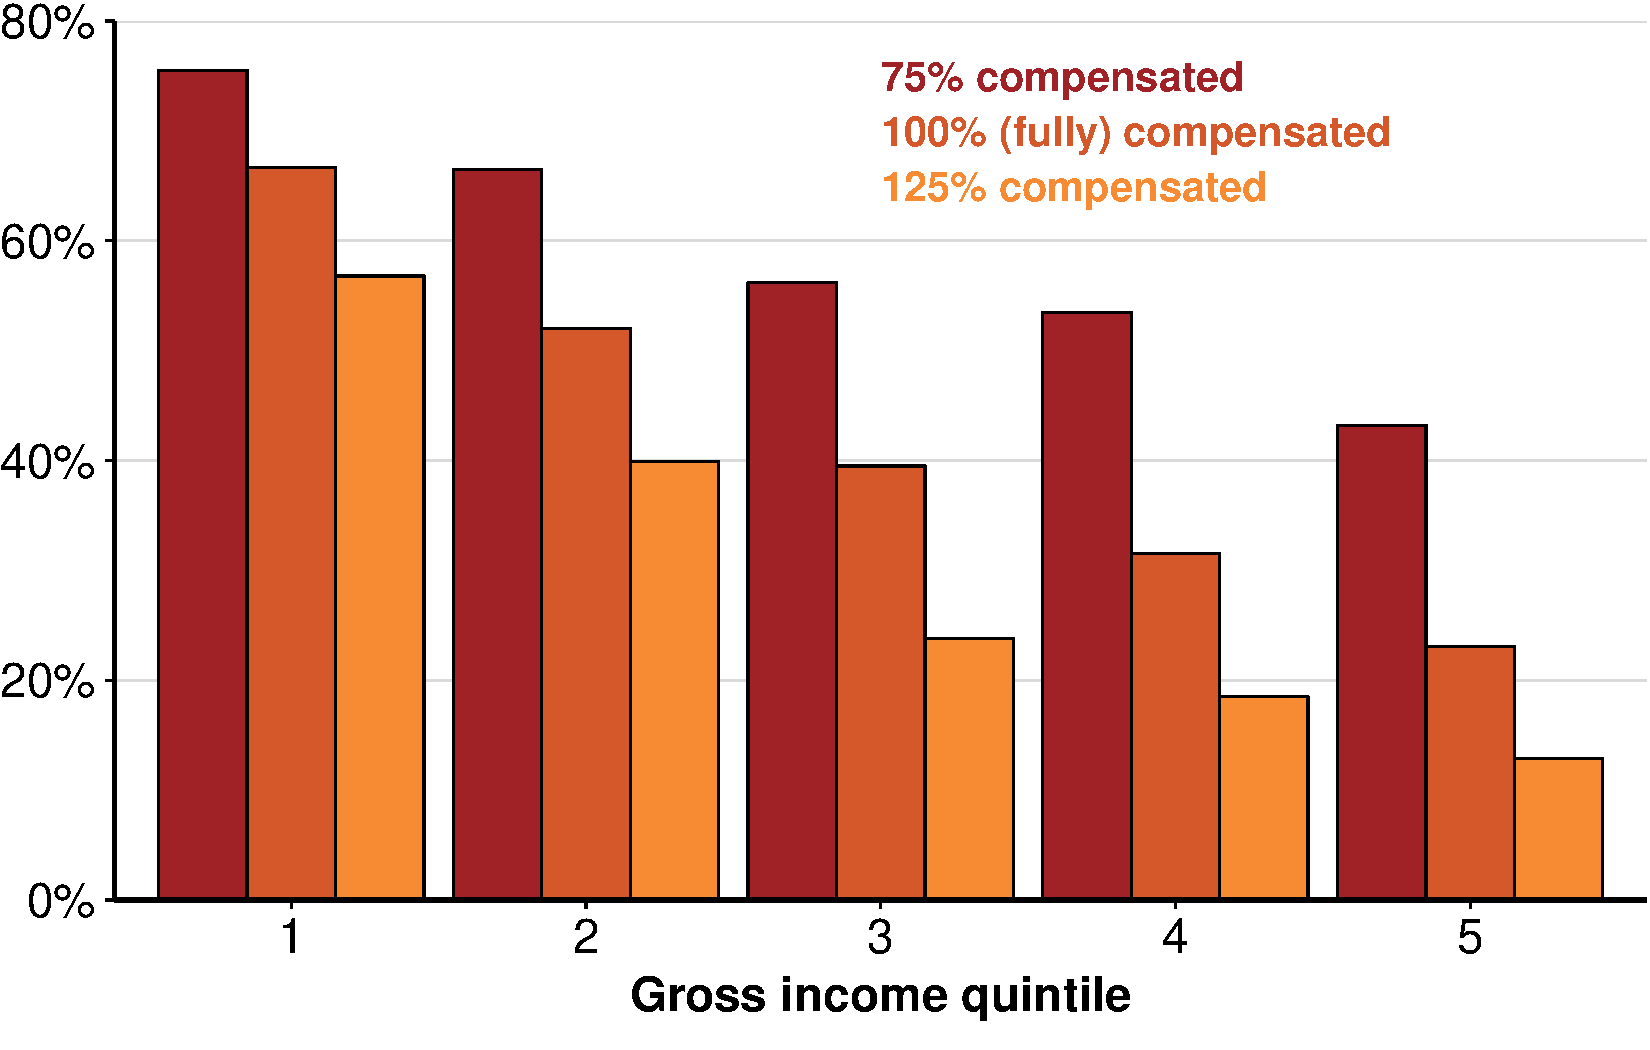
\includegraphics[width=11.000in,height=7.00in]{figure/GST-Figure-9-1} 

\end{knitrout}

\begin{knitrout}
\definecolor{shadecolor}{rgb}{0.969, 0.969, 0.969}\color{fgcolor}
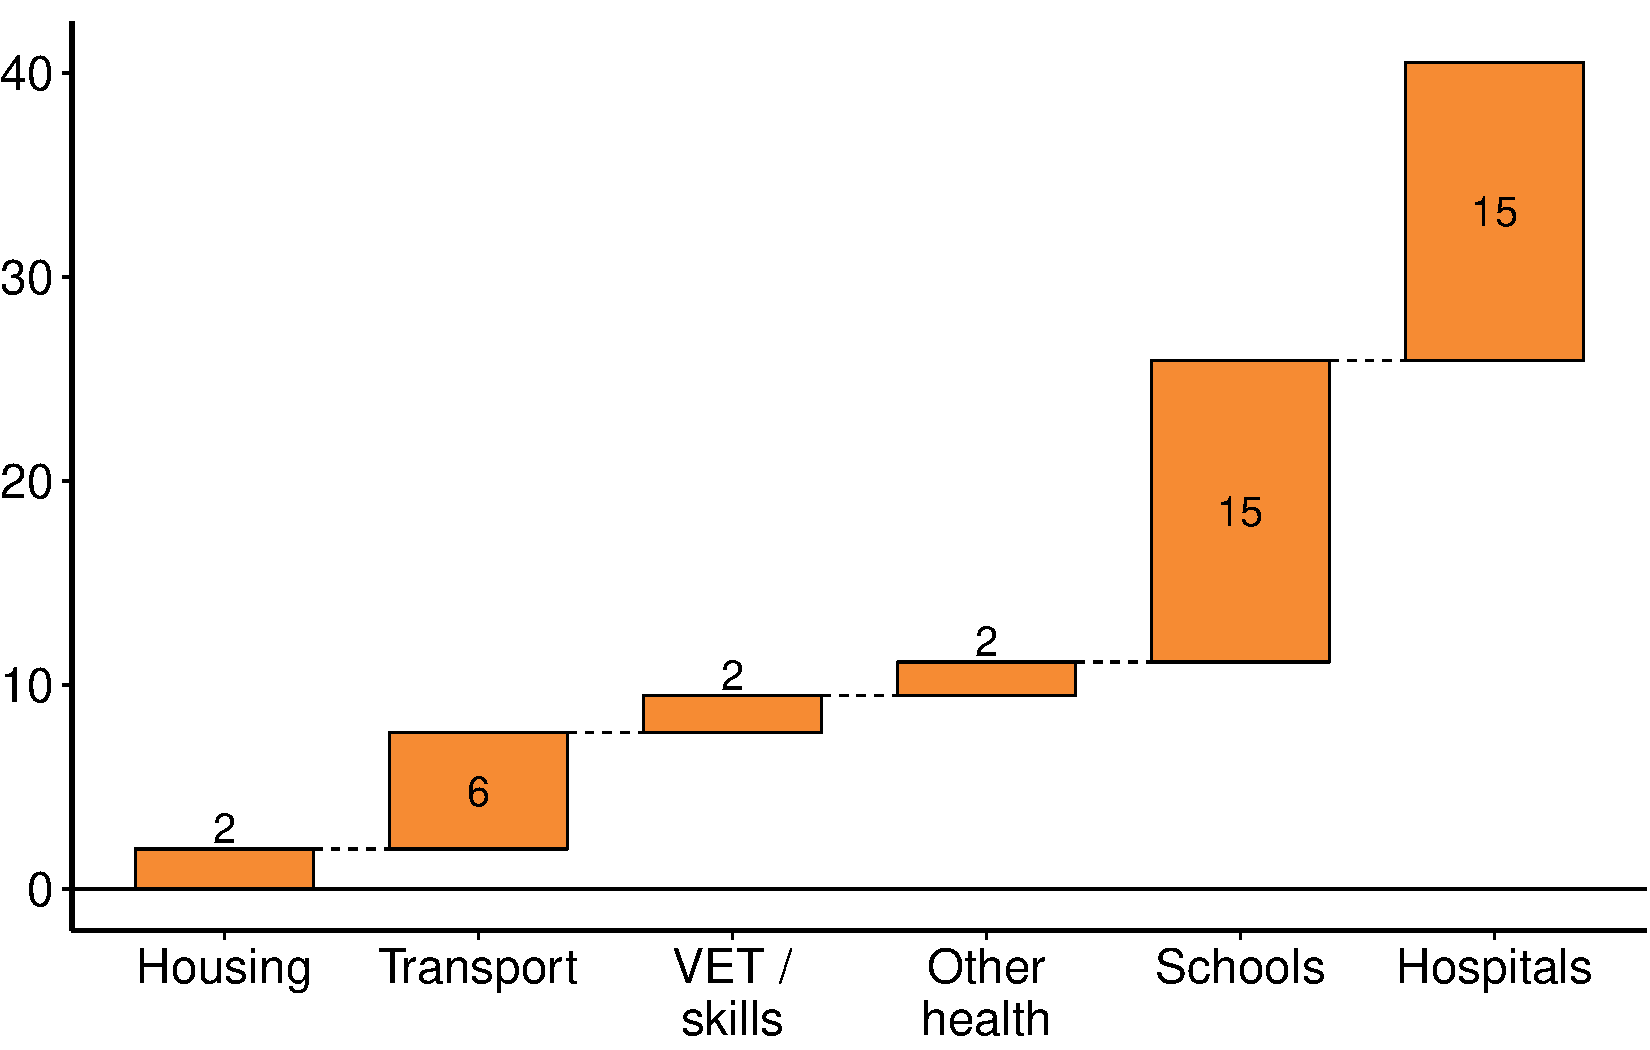
\includegraphics[width=11.000in,height=7.00in]{figure/GST-Figure-10-1} 

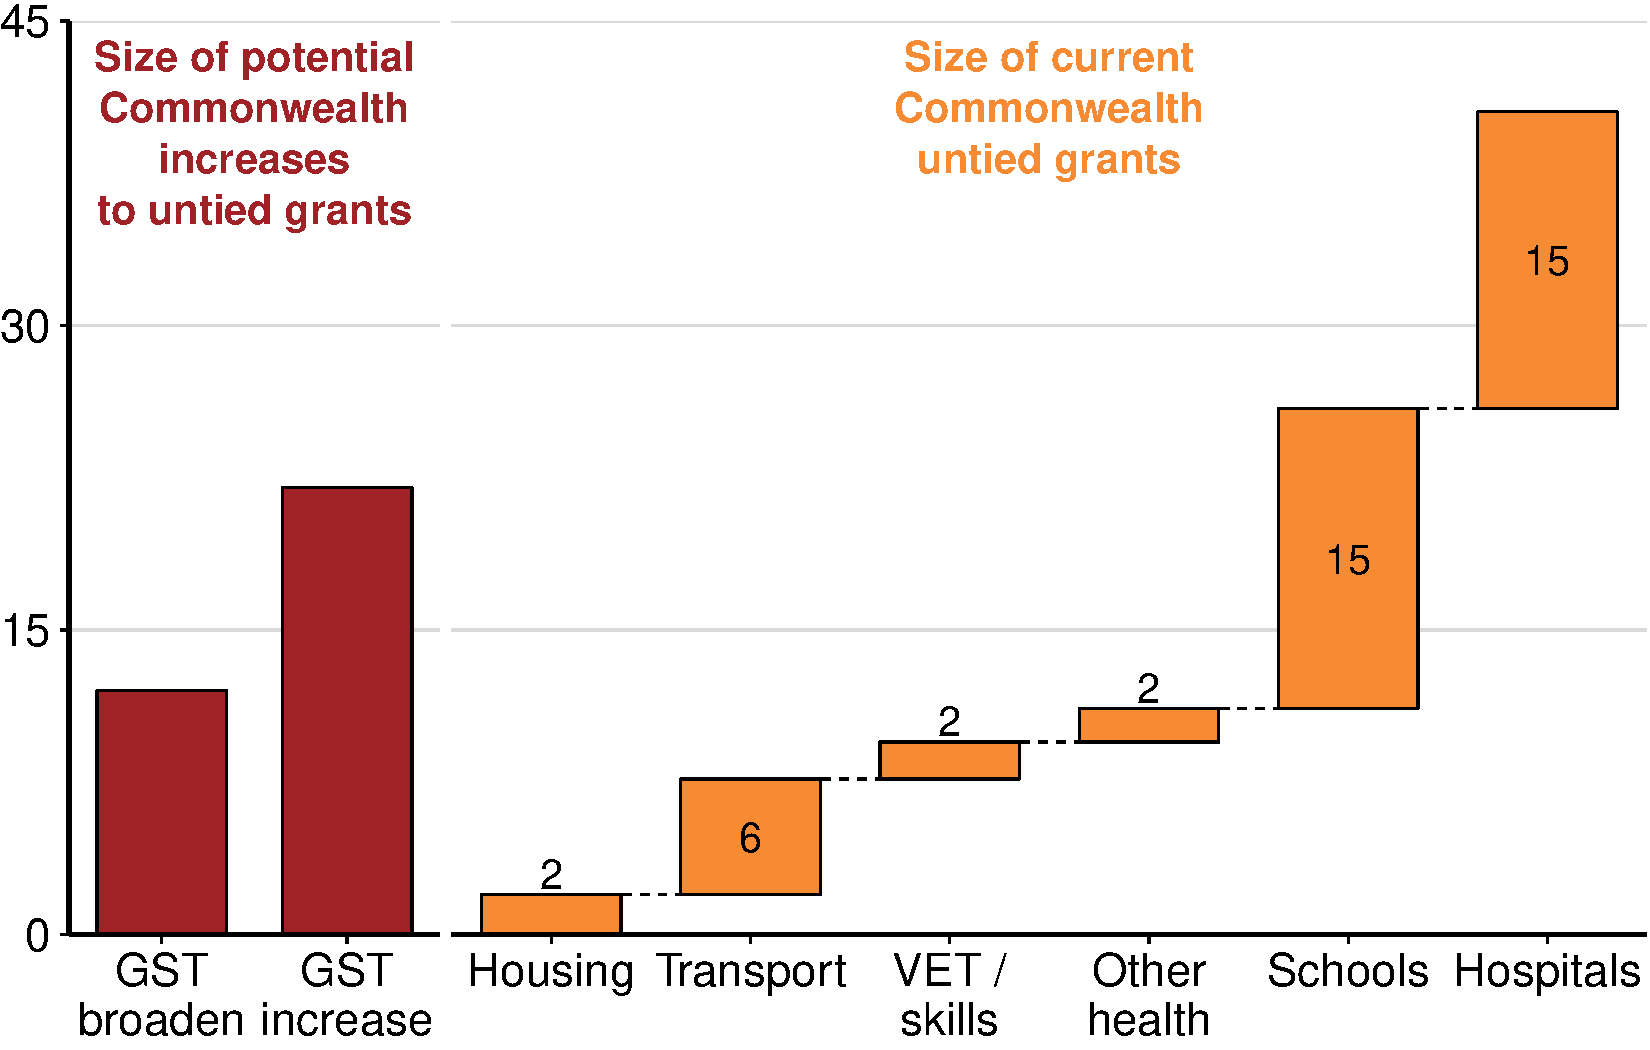
\includegraphics[width=11.000in,height=7.00in]{figure/GST-Figure-10-2} 

\end{knitrout}

\begin{knitrout}
\definecolor{shadecolor}{rgb}{0.969, 0.969, 0.969}\color{fgcolor}
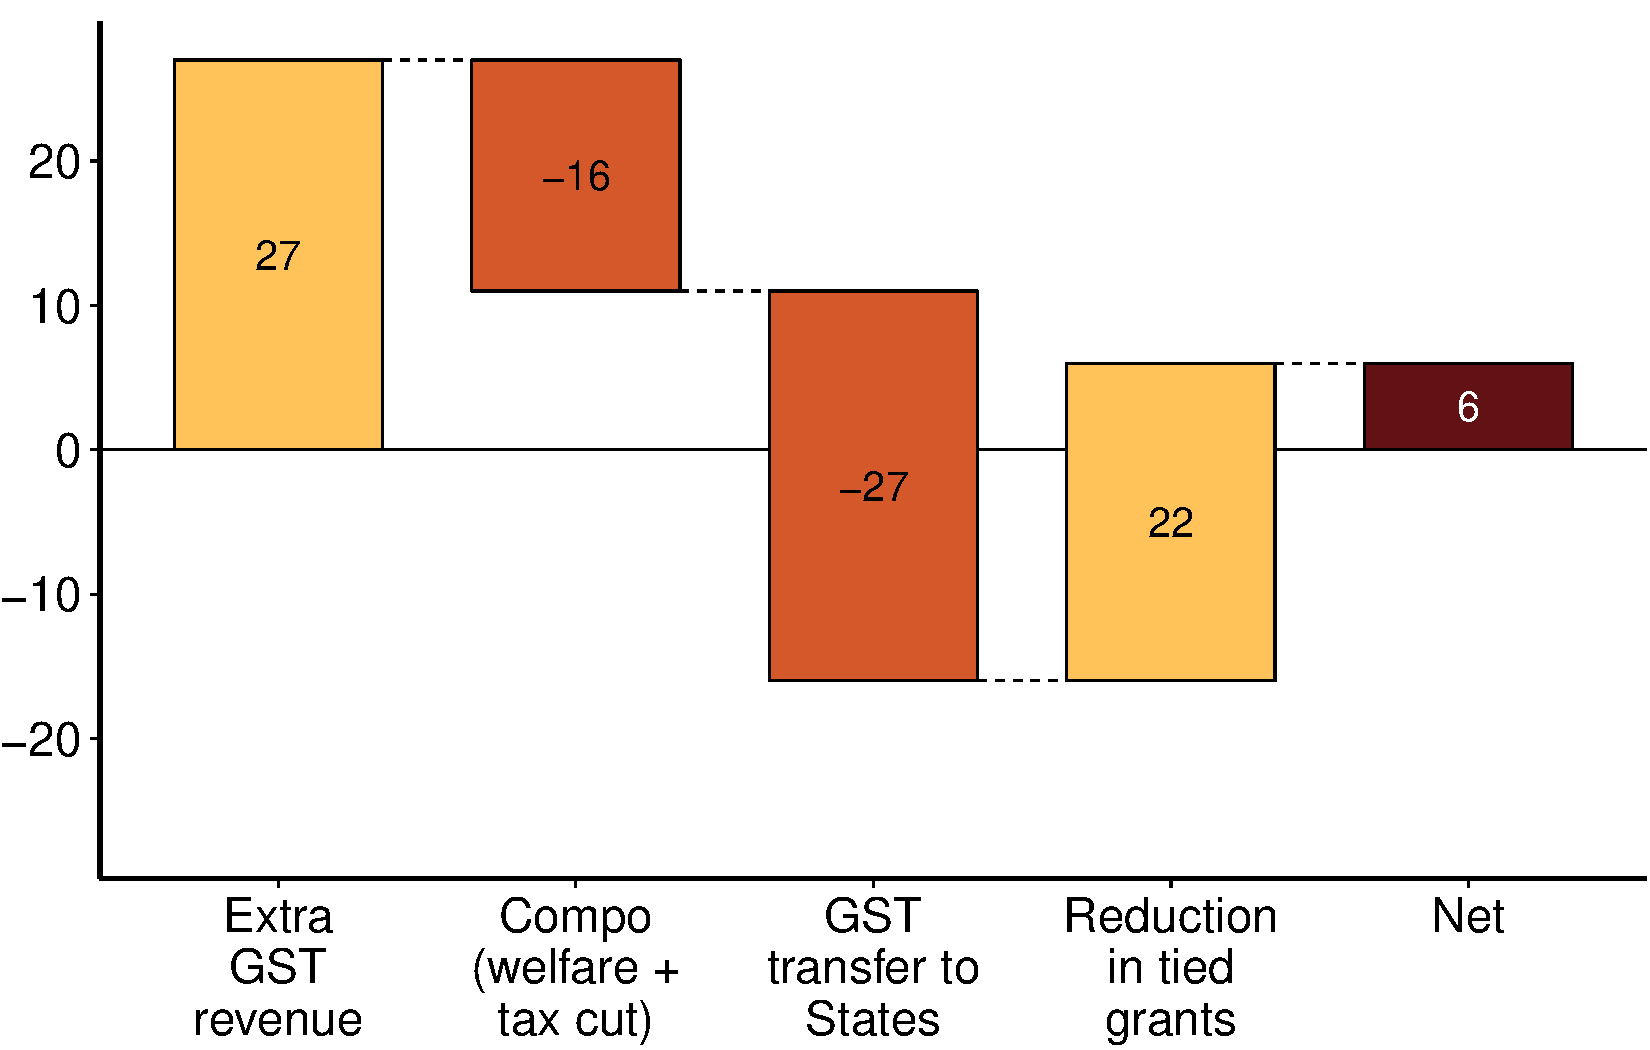
\includegraphics[width=11.000in,height=7.00in]{figure/GST-Figure-11-1} 

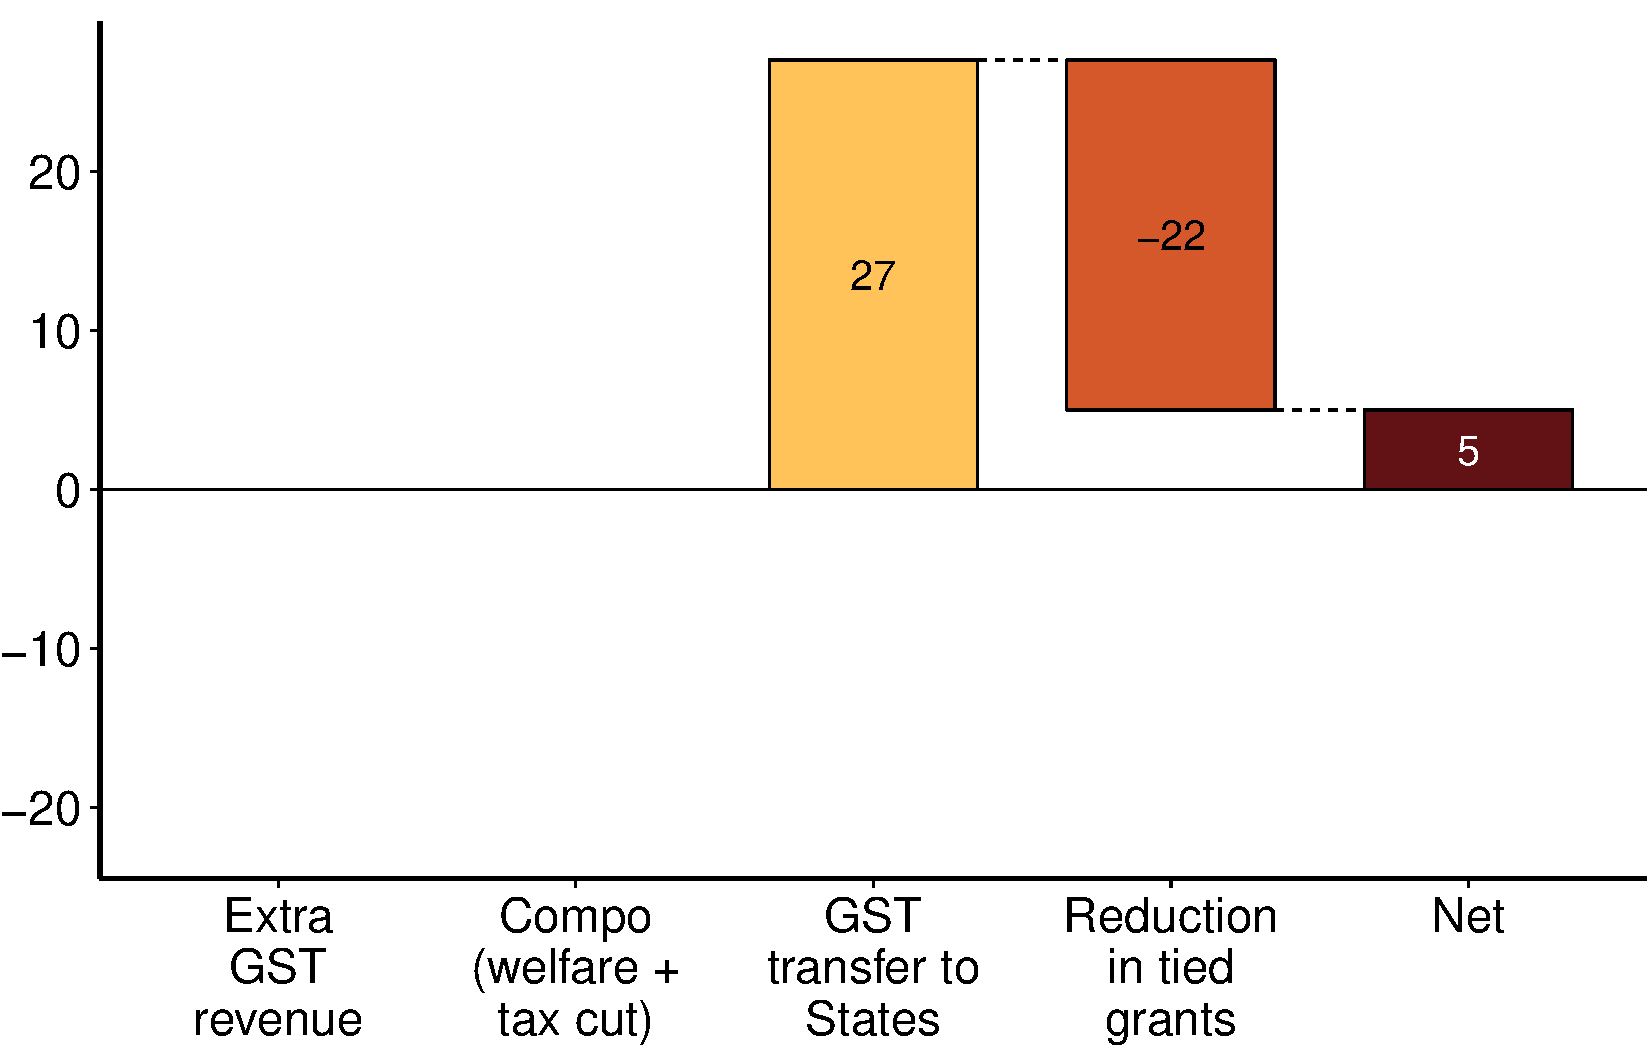
\includegraphics[width=11.000in,height=7.00in]{figure/GST-Figure-11-2} 

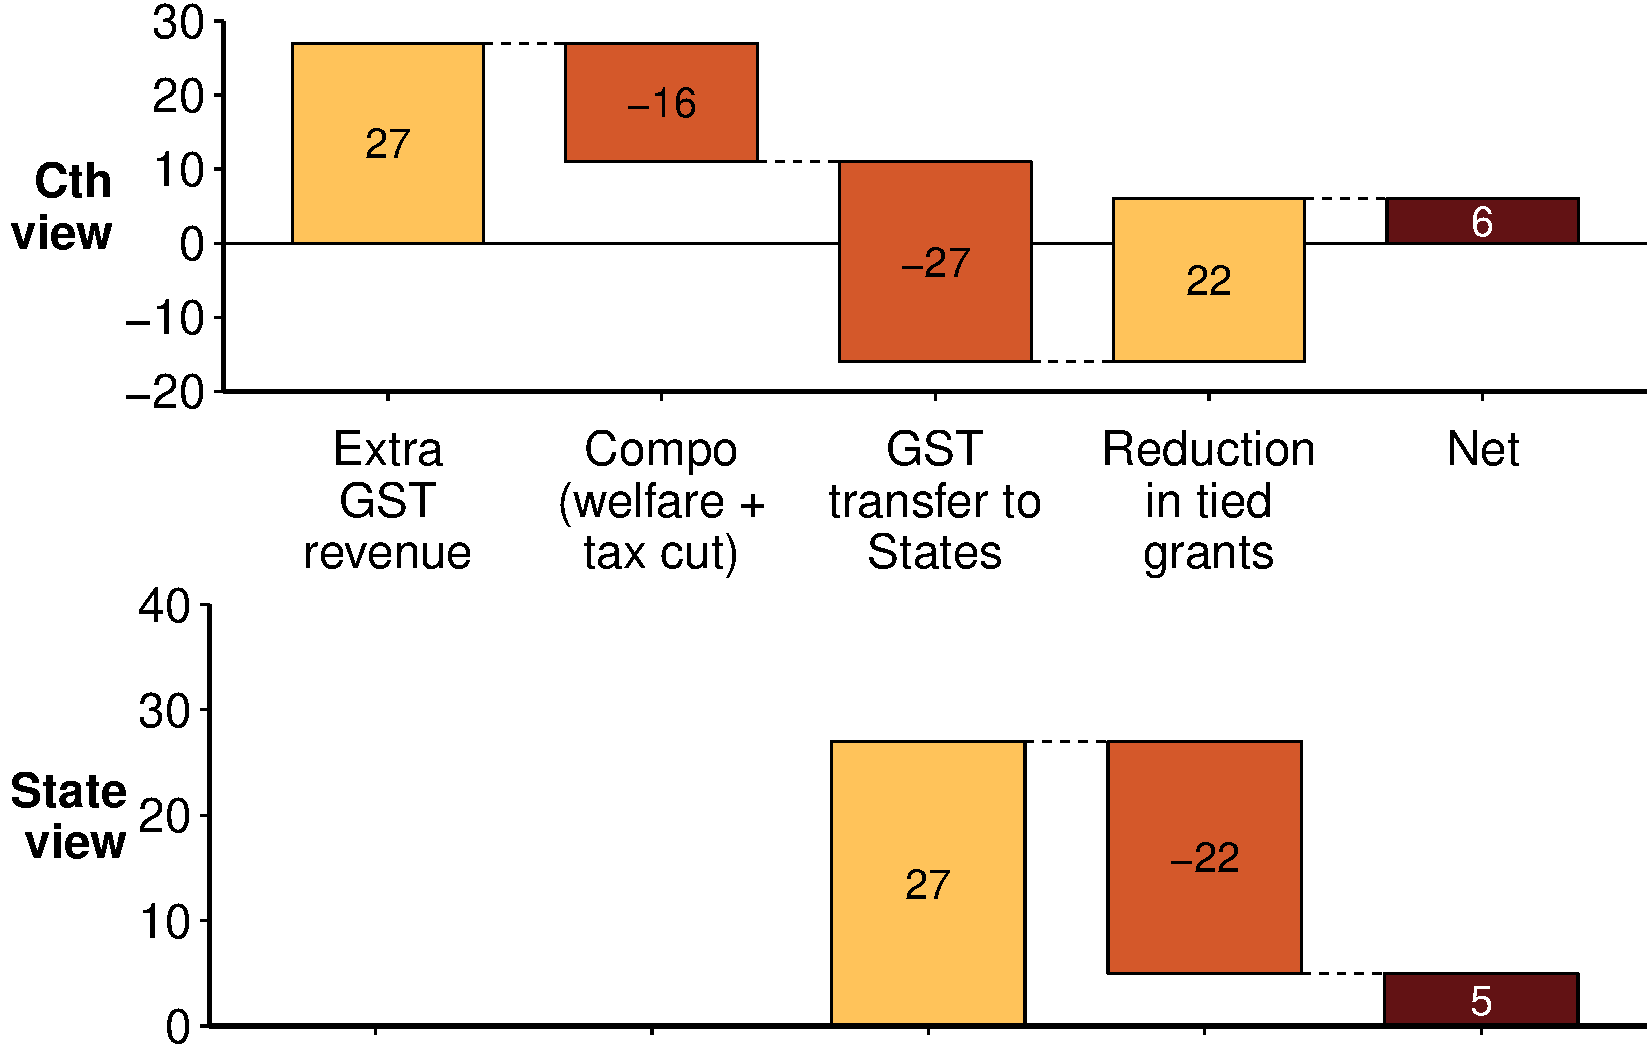
\includegraphics[width=11.000in,height=7.00in]{figure/GST-Figure-11-3} 

\end{knitrout}

\begin{knitrout}
\definecolor{shadecolor}{rgb}{0.969, 0.969, 0.969}\color{fgcolor}
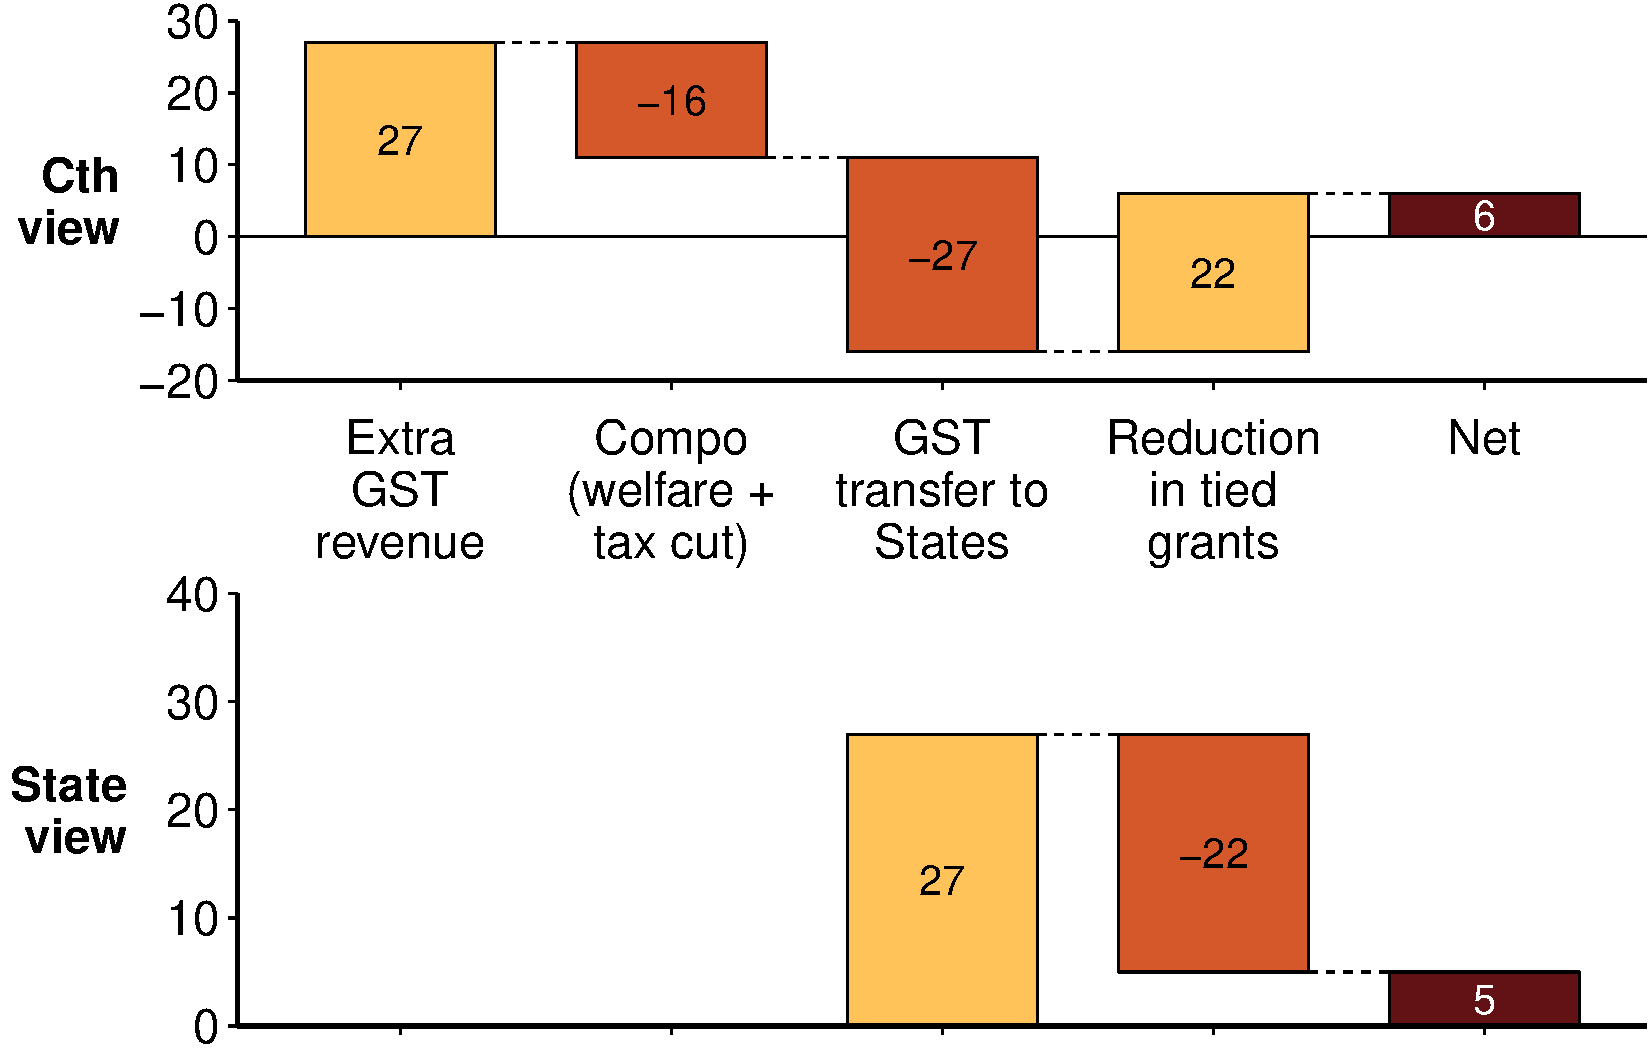
\includegraphics[width=11.000in,height=7.00in]{figure/cowplot-1} 

\end{knitrout}



\begin{knitrout}
\definecolor{shadecolor}{rgb}{0.969, 0.969, 0.969}\color{fgcolor}\begin{kframe}
\begin{verbatim}
## TableGrob (6 x 5) "layout": 8 grobs
##   z     cells       name                                    grob
## 1 0 (1-6,1-5) background zeroGrob[plot.background..zeroGrob.740]
## 2 3 (3-3,3-3)     axis-l     absoluteGrob[GRID.absoluteGrob.734]
## 3 1 (4-4,3-3)     spacer                          zeroGrob[NULL]
## 4 2 (3-3,4-4)      panel                   gTree[GRID.gTree.718]
## 5 4 (4-4,4-4)     axis-b     absoluteGrob[GRID.absoluteGrob.726]
## 6 5 (5-5,4-4)       xlab    zeroGrob[axis.title.x..zeroGrob.735]
## 7 6 (3-3,2-2)       ylab  titleGrob[axis.title.y..titleGrob.738]
## 8 7 (2-2,4-4)      title      zeroGrob[plot.title..zeroGrob.739]
## TableGrob (6 x 5) "layout": 8 grobs
##   z     cells       name                                    grob
## 1 0 (1-6,1-5) background zeroGrob[plot.background..zeroGrob.787]
## 2 3 (3-3,3-3)     axis-l     absoluteGrob[GRID.absoluteGrob.781]
## 3 1 (4-4,3-3)     spacer                          zeroGrob[NULL]
## 4 2 (3-3,4-4)      panel                   gTree[GRID.gTree.767]
## 5 4 (4-4,4-4)     axis-b     absoluteGrob[GRID.absoluteGrob.773]
## 6 5 (5-5,4-4)       xlab    zeroGrob[axis.title.x..zeroGrob.782]
## 7 6 (3-3,2-2)       ylab  titleGrob[axis.title.y..titleGrob.785]
## 8 7 (2-2,4-4)      title      zeroGrob[plot.title..zeroGrob.786]
\end{verbatim}
\end{kframe}
\end{knitrout}

\phantom{.}




\end{document}
